\documentclass[12pt]{article}
\usepackage{listings}
\usepackage{url}
\usepackage{placeins}
\usepackage[paper=letterpaper,
           marginparwidth=1in,
           hmargin={1.1in,0in},
           vmargin={1in,1.5in},           
           includemp
           ]{geometry}
           
 \usepackage{longtable}
 \usepackage{graphicx}
 \usepackage{caption}
\usepackage{subcaption}
\usepackage[]{natbib}
\usepackage{latexsym,amsfonts,amssymb,amsmath,amsthm,mathrsfs}
\usepackage{bbm}
\usepackage{amsthm}
\newtheorem{definition}{Definition}
\usepackage{hyperref}
\usepackage{lscape}

\hypersetup{
    bookmarks=true,         % show bookmarks bar?
    unicode=false,          % non-Latin characters in Acrobat’s bookmarks
    pdftoolbar=true,        % show Acrobat’s toolbar?
    pdfmenubar=true,        % show Acrobat’s menu?
    pdffitwindow=false,     % window fit to page when opened
    pdfstartview={FitH},    % fits the width of the page to the window
    pdftitle={My title},    % title
    pdfauthor={Author},     % author
    pdfsubject={Subject},   % subject of the document
    pdfcreator={Creator},   % creator of the document
    pdfproducer={Producer}, % producer of the document
    pdfkeywords={keyword1} {key2} {key3}, % list of keywords
    pdfnewwindow=true,      % links in new window
    colorlinks=true,       % false: boxed links; true: colored links
    linkcolor=red,          % color of internal links (change box color with linkbordercolor)
    citecolor=black,        % color of links to bibliography
    filecolor=magenta,      % color of file links
    urlcolor=blue           % color of external links
}
\providecommand{\keywords}[1]{\textbf{\textit{Keywords ---}} #1}


\begin{document}
\title{Final Project: Implementation of PSRL and UCRL in the RLPy platform}
\date{March 18, 2015}
\author{Imanol Arrieta Ibarra}
\maketitle

\begin{abstract}
RLPy is a python library that implements several Reinforcement Learning algorithms in an object-oriented environment. By incorporating UCRL and PSRL to this platform, I am able to easily compare these algorithms across a great gamma of already implemented domains. In the following document I will compare PSRL, UCRL, SARSA and LSPI across two domains. The first is a classic MDP chain problem and the second one is the solution of a labyrinth. 
\end{abstract}

\section{Introduction}
According to \cite{RLPy}: ``RLPy is a framework for conducting sequential decision making experiments involving value-function based approaches. It provides a modular toolbox, where various components can be linked together to create experiments.'' Although this platform is intended to evaluate value-function based approaches, in the following sections I'll explain how I programmed two model based approaches in this environment. The result is the potential to compare both PSRL and UCRL against a great variety of already implemented Reinforcement Learning Methods. 

In section \ref{sec:platform} I'll introduce the RLPy platform together with the elements that compose it. In section \ref{sec:alg} I'll reference the different algorithms used to exemplify the potential of implementing PSRL and UCRL to RLPy. Sections \ref{sec:mdp} and \ref{sec:grid} show two examples of domains which are useful to compare the different algorithms. Finally, I conclude in section \ref{sec:conc}.

All the code developed for this project can be found in the github repository: \url{https://github.com/imanolarrieta/RL.git}. The specific files for implementing UCRL and PSRL are located in: rlpy/Agents/UCRL and rlpy/Agents/PosteriorSampling correspondingly. 



\section{The platform}
\label{sec:platform}
The RLPy platform \citep{RLPy} consists mainly of five modules which, when put together, allow users to create experiments. Figure \ref{fig:RLPy} broadly shows how these modules interact. In the following subsections, I will give a short description of each module.

\begin{figure}[h]
\centering
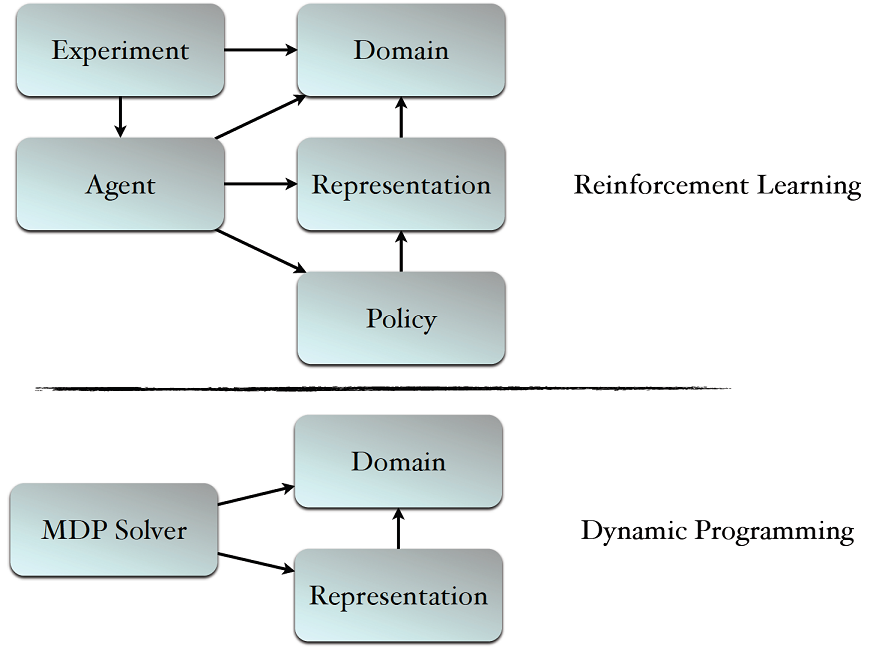
\includegraphics[trim=0cm 7cm 0cm 0cm, clip=true, scale=.4]{platform.png}
\caption{Reinforcement Learning scheme of RLPy}
\label{fig:RLPy}
\end{figure}

\subsection{Agent}
An agent is the module where the learning takes place. For the case of the RLPy original algorithms, it updates the weight vector corresponding to the features \citep{RLPy}. For the case of PSRL and UCRL, it will record for each (state,action):
\begin{itemize}
\item The mean of the rewards.
\item The variance of the rewards.
\item The number of times the pair has been observed.
\item The number of times a given new state is observed.
\end{itemize}
Then, at the end of each episode it will select a model according to the particular algorithm and will store the model.

In total there are six agents already programmed:
\begin{enumerate}
\item Q Learning
\item SARSA
\item Greedy GQ
\item LSPI
\item LSPI-SARSA
\item Natural Actor Critic
\end{enumerate}

The contribution of this project is to include PSRL and UCRL to this list.
\subsection{Domain}

A domain is the particular MDP we want to solve \citep{RLPy}. In total 24 domains have already been programmed in RLPy. This makes this platform extremely rich to test new algorithms, and is the main motivation to implement PSRL and UCRL to it. However, not all of these domains will be useful. Their usefulness will depend in the number of states these domains define. Since RLPy takes advantage of linear Q-function approximation, this limitation does not apply for the originally implemented algorithms.

Some examples of domains are:
\begin{enumerate}
\item GridWorld
\item Chain MDP
\item Pacman
\end{enumerate}

In this project I will limit myself to test PSRL and UCRL only on the first two domains.
\subsection{Representation}
RLPy assumes that linear function approximations are used to represent the value function. This module defines the representation used for capturing the value function \citep{RLPy}. This is, it defines the features used to represent each domain. 

There are 15 representations in RLPy. Of unique interest to us is a representation called Tabular. This provides no generalization in that each feature takes the following form:
$$\Phi_s(x) = \left\lbrace \begin{array}{lr}
1 & :x=s\\
0 & o.w. 
\end{array} \right.$$
This means that for each state we get a feature. This is why in many domains we will not be able to apply UCRL or PSRL. The number of states may be prohibitive.
 
\subsection{Policy}
This module is responsible to generate actions based on current states \citep{RLPy}.There are six policies implemented in RLPy:
\begin{enumerate}
\item Epsilon Greedy
\item Fixed Policy
\item Uniform Random
\item Gibbs Policy
\item Fixed Policy
\item Basic Puddle Policy
\end{enumerate}
From these we will only consider the Epsilon Greedy one because we can always define epsilon as zero.

\subsection{Experiment}
An experiment is the main module of the platform. This is the module that connects all other ones and solves the problem \citep{RLPy}. Each experiment consists on the creation of an instance of each of the previous models. After creating several experiments, RLPy allows users to compare output between them and, as so, compare the efficacy and efficiency of different kinds of modules.

\subsection{Experiment Evaluation}
\cite{RLPy} defined a particular way of evaluating an experiment which is completely intuitive and easy to implement for value-function based approaches, but which is not particularly well fitted to evaluate PSRL and UCRL. A useful continuation of this project could be the programming of an evaluation metric such as regret over the realized episodes. This is not straightforward since that part of the platform is actually somewhat buggy and badly documented.

If we consider an experiment consisting of L episodes, instead of evaluating the policy function at each episode, \cite{RLPy} evaluate only certain episodes. \cite{RLPy} choose $l$ equally separated episodes and conduct what they call learning steps. For example, if we have an experiment consisting of a thousand episodes and are interested in 10 learning steps, we would evaluate only every 100th episode. Then, a learning step would consist of taking one of the selected episodes, stop exploration (for the case of value function approaches this usually means making $\epsilon=0$), and run $m$ policy checks. Each policy check consists of running an episode with no exploration. Then we take the average reward of the $m$ policy checks as our performance measure for the given learning step.

One issue with UCRL and PSRL is that it is not evident how to stop exploration. For PSRL we could concentrate the posterior probability in the mean and for USRL we could take the middle point of the confidence interval. But it does not seem clear that this would be equivalent to no exploration. Also, for the way the RLPy library is structured, stopping exploration in UCRL and PSRL would involve changing the original source code for the library. The reason for this is that exploration takes place in the Agent module for PSRL and UCRL, while for all other methods it takes place in the Policy stage. For this reason, the RLPy library only deals with stopping exploration in the Policy module and actually never calls the Agent when evaluating. 



\section{Algorithms}
\label{sec:alg}

\subsection{UCRL}
Upper Confidence for Reinforcement Learning is a model-based algorithm introduced by \cite{UCRL}. It consists on building confidence sets over the transition probabilities' and rewards' models and then choosing the one which provides the greatest sum of expected rewards.
\subsection{PSRL}
Posterior Sampling for Reinforcement Learning was introduced by \cite{PSRL}. It is a model-based approach based in sampling transition probability and reward models from a posterior distribution. This method is inspired in Thompson Sampling and works as an optimal approximation to UCRL. 

\subsection{SARSA}
Described in \cite{Sutton} is a value function based algorithm that updates the $Q$-function the following way: $$Q(s_t,a_t) \leftarrow Q(s_t,a_t) + \alpha [r_{t+1} + \gamma Q(s_{t+1}, a_{t+1})-Q(s_t,a_t)]$$
$\alpha$ is a learning parameter and $\gamma$ is a discount parameter. For exploration, RLPy uses an epsilon-greedy approach.

\subsection{LSPI}
Least Squares Policy Iteration is a model free algorithm which combines least squares function approximation with policy iteration. Presented by \cite{LSPI}, this method explores in the RLPy framework using epsilon-greedy.

\section{MDP Chain}
\label{sec:mdp}

This experiment consists of a chain of $n$ nodes. There are $n$  states, each one representing the presence of the agent in one of the $n$ nodes. At each point in time, the agent has access to two possible actions: left or right. By choosing an action, the agent moves deterministically in the direction of the action except for the first node when choosing left and the last node when choosing right. For these cases the agent remains in the same node. The rewards for each state are -1 except the last node which gives a reward of 0. Each episode takes $2n$ time periods or the number of steps it takes to arrive to the last node. Mathematically the experiment consists of the following objects:
\begin{equation}
\begin{array}{rl}
\text{(number of steps per episode)} & T = \textit{min}(\text{number of states to arrive at state n},2n)\\
\text{(states)}&S = \{1,2,..., n\}\\
\text{(actions)} &A = \{-1,1\}\\
\text{(transitions)} & s_{t+1}(s_t,a_t) = max\{0,min\{n,s_t+a_t\}\}\\
\text{(rewards)}& r(s,a) = \left\lbrace \begin{array}{lr}
-1 & : s_{t+1}<n\\
0 & :s_{t+1}=n
\end{array} \right.
\end{array}
\end{equation}

For the experiments I tested, I only considered $n=10$ which means the maximum number of steps would be $20$. 

\subsection{Optimal Performance}

The optimum reward for each episode should be $n-2$ , so, for the case of $n=10$ the best possible return should be $-8$.

\subsection{Results}

 Figure \ref{fig:res_mdp} shows how the different algorithms performed on this domain. Each line is the average over 5 different runs, the shadow area around the line represents the confidence interval. In the previous graph UCRL attains the same velocity of convergence as LPSI and SARSA. PSRL converges but only after some extra exploration. In the end, all algorithms attain optimal rewards. It is strange that PSRL performs so much worse than the other algorithms. I have run the experiment with different reward structures and obtained the same results. One possibility is that the way PSRL is encoded is incompatible with some part of the evaluation process that I am overlooking. The evaluation code for RLPy is extremely obscure and inconsistent. As I said before, it may be worthwhile to encode other types of evaluations in order to fix this problem.

\begin{figure}[h]
\centering
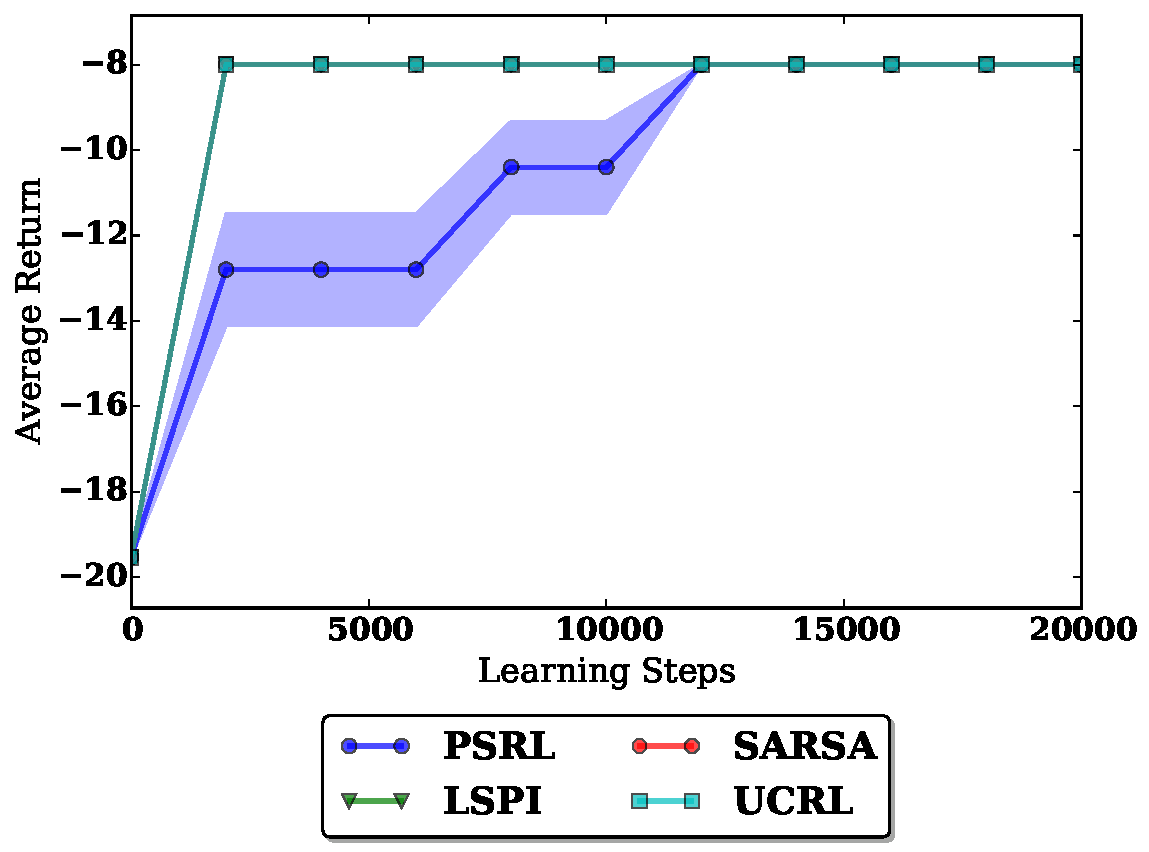
\includegraphics[scale=.4]{MDP.pdf}
\caption{Average Return for the MDP chain}
\label{fig:res_mdp}
\end{figure}


\FloatBarrier
\section{GridWorld}
\label{sec:grid}
This experiment consists on a labyrinth with two pits and an exit. The agent starts at the beginning of the labyrinth and moves until it walks the maximum number of steps, encounters a pit or reaches the end. Figure \ref{fig:GW} shows how the labyrinth looks like. The blue square corresponds to the starting point, the red ones to the pits, the gray ones to the walls and the green one to the exit.

Given a labyrinth of $m*n$, the number of states is $m*n$. If we consider a matrix with $m$ rows and $n$ columns, each state would correspond to an entry of the matrix. The agent could potentially be in any of the entries.

The agent starts in the matrix entry represented by the blue square. Then, at each point in time, it can choose to move left, up, right or down . The episode lasts either 1000 steps or the number of steps it takes to get to a pit or to the exit of the maze ( green or red squares)

For this experiment, the original RLPy representation of the domain would indicate the agent which actions were possible at each state. This means that by default the agent would not be able to observe certain states resulting in terrible results for PSRL and UCRL. I could encode this in the prior for PSRL or a in the domain representation for both algorithms, taking away states that were never visited, but this would mean that the user has some knowledge about the structure of the maze. Since I wanted the agent to discover the maze by itself, I made a modification in both algorithms. At each state, I will consider every non-available action. For this actions I will register them as if the agent has observed them with a terrible reward and a deterministic transition to the same state. This way it would take very little passes for the algorithm not to take the unavailable states into account when choosing optimistic models.

In mathematical terms, this experiment consists in the following objects:

\begin{equation}
\begin{array}{rl}
\text{(number of steps per episode)} & T = \textit{min}(\text{number of states to arrive at (3,1) or (3,2)},1000)\\
\text{(states)}&S = \{(0,0),(1,0),...,(3,4)\}\\
\text{(actions)} &A = \{(0,-1),(-1,0),(0,1),(1,0)\}\\
\text{(transitions)} &  s_{t+1} = s_t+x \quad \text{for} \quad x\in A(s_t)\\
\text{(rewards)}& r(s,a) = \left\lbrace \begin{array}{lr}
-1 & :  s_{t+1}\in \{(3,1),(3,2)\}\\
1 & :s_{t+1}=(3,3)\\
-0.001 & : o.w.

\end{array} \right.
\end{array}
\end{equation}

\subsection{Optimal Performance}
We will take only into account the maze described in figure \ref{fig:GW}. Since the maximum number of steps is $1000$, the optimal policy should give back a reward of $0.99$.
\begin{figure}[h]
\centering
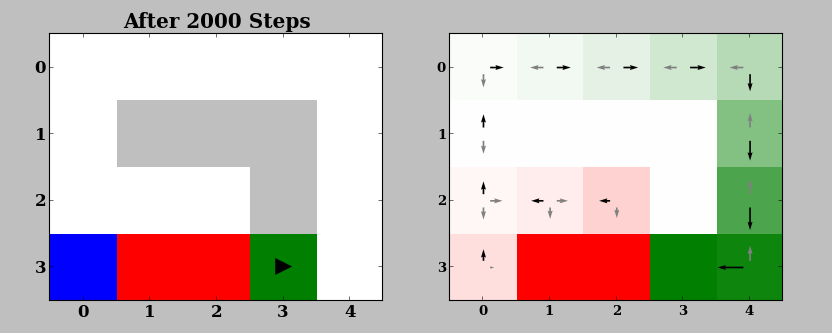
\includegraphics[trim=0cm 0cm 0cm 1.1cm, clip=true, scale=.4]{gridWorld.png}
\caption{GridWorld labyrinth and example of policy}
\label{fig:GW}
\end{figure}


\subsection{Results}

 Figure \ref{fig:res_mdp} shows how the different algorithms performed on this domain. Each line is the average over 5 different runs, the shadow area around the line represents the confidence interval. I could not run UCRL over a large number of steps for the amount of time it took. While the other algorithms took a matter of minutes, UCRL was taking more than three days. Nevertheless, even at 50,000 steps it seemed that UCRL was having trouble converging. Giving the results a closer look, it seems that there may be some incompatibility between the way PSRL and UCRL are encoded and the way the learning steps are computed. While running, the normal steps look much better than the ones taken from the learning steps episodes. As stated before, this is one of the most obscure pieces of code from RLPy and from all I can see there does not appear to be a bug. Either way by encoding a different type of evaluation I could be able to solve both problems at once.




\begin{figure}[h]
\centering
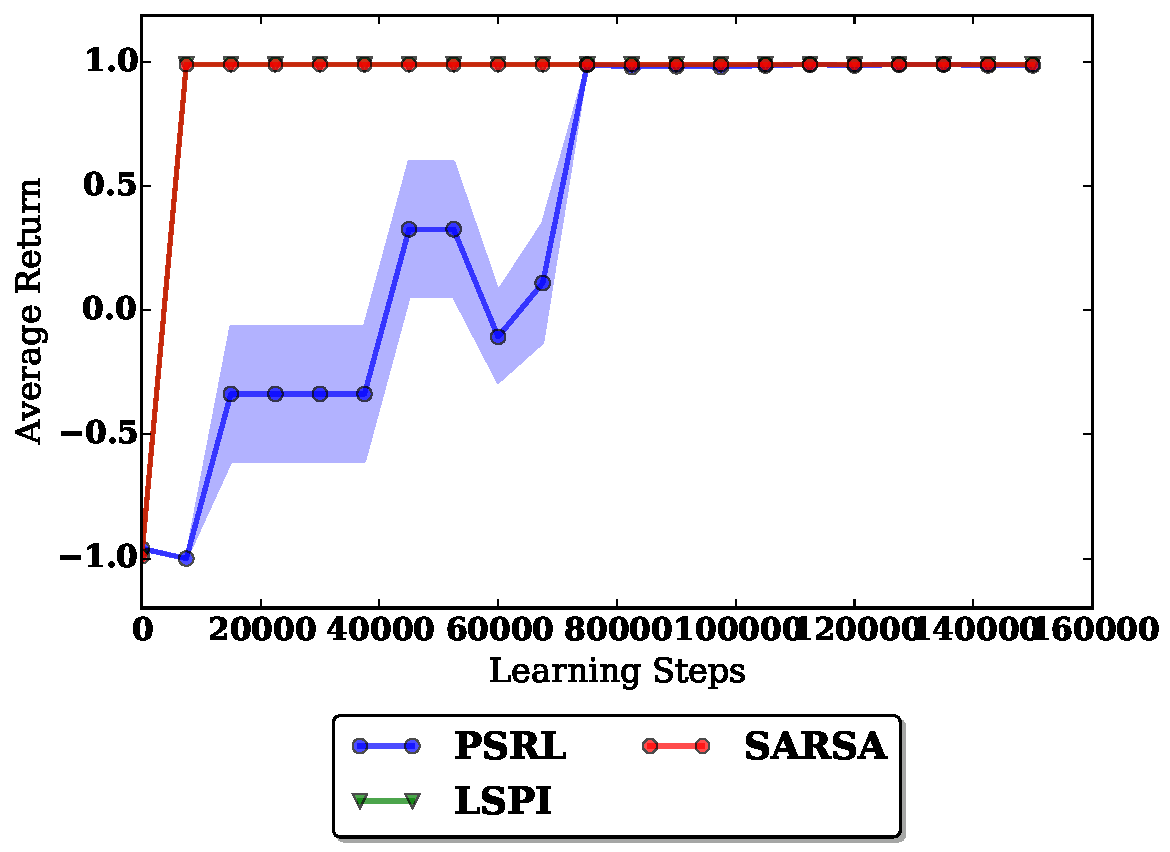
\includegraphics[scale=.4]{Grid.pdf}
\caption{Average Return for GridWorld}
\label{fig:res_grid}
\end{figure}


\section{Conclusions}
\label{sec:conc}
These are some of the examples in which we would be able to test PSRL and UCRL. The only disadvantage, and the reason why I am not presenting any more at the moment is that, because of Python limitations, the implementation of PSRL and UCRL can not be properly vectorized and, because of this, runs extremely slow. To run the two previous simulations it took about 8 hours for the MDP chain and 3 days for gridworld, even though I was performing all computations in parallel. However, if time is not a constraint, having this two algorithms on RLPy provides great opportunity to compare them to value function based algorithms.

There is still plenty of work to make the integration of PSRL and UCRL with RLPy a useful one. Sampling from distributions in python is very costly, looking for ways to speed up this process could really help the implementation of these algorithms. On the evaluation side, \cite{RLPy}'s approach could be improved by adding further measures. This would involve changes to the original source code but would greatly benefit the whole platform. 

I have thoroughly checked for bugs in my code, and during the learning phases, both UCRL and PSRL seem to be doing fine. The bad performance comes up only at the evaluation learning steps. This is why I believe that there must be something incompatible between the way PSRL and UCRL were encoded and the evaluation code. In the end I had to implement many operations that go against the RLPy  paradigm of value-function approaches. However, even when running the already implemented algorithms I encountered problems in the way RLPy does evaluation. 

To sum up, I coded the PSRL and UCRL algorithms to the RLPy platform, opening up a great opportunity to compare these against previously encoded algorithms. There is still work to be done to make the evaluation of these algorithms coherent but it should not be too complicated to do that.
\newpage

\bibliographystyle{chicago}
\bibliography{biblio}



\end{document}